\chapter{Sheaves}
\section{Topological Presheaves and Sheaves}

Let $X$ be a topological space. Denote the set of open subsets of $X$
as $\textbf{Open}(X)$. We can impose the structure of a
\hyperref[definition:thin-category]{\textcolor{Blue}{thin category}}
on this set by declaring that, for two open sets $U$ and $V$, 
\[
    \hom_{\textbf{Open}(X)}(U, V) = 
    \begin{cases}
        \{\bullet\} & \text{if } U \subset V\\
        \varnothing & \text{otherwise }
    \end{cases}
\]
That is, we allow a single morphism from $U$ to $V$ if and only if 
$U \subset V$. 
Now suppose $Y$ is another topological space. Then for each open subset 
$U$ of $X$ we may construct the set 
\[
    C(U) = \{ f: U \to Y \mid f \text{ is continuous } \}.    
\]
Observe that if $U \subset V \subset X$ are open sets, then 
there is function 
\[
    \rho_U^V: C(V) \to C(U)
\]
where each $f: V \to Y$ is mapped to its restriction $f|_U: U \to Y$.
What follows is an important observation: If we have a chain of three open subsets $U \subset V \subset W$, 
then any continuous function $f: W \to Y$ can be restricted to $f|_V: V \to Y$, 
which can then be restricted to $f|_V|_U: U \to Y$. However, we obtain the same 
result if we instead just restrict $f$ to $U$ in the first place. That is, 
$f|_V|_U = f|_U$. In our notation, this implies that 
\[
    \rho_V^W \circ \rho_U^V = \rho_U^W. 
\]
What we have on our hands is a \emph{contravariant} functor (since the relation 
$U \subset V$ induces a function $C(V) \to C(U)$). As covariant functors 
are easier to think about, we can equivalently express this as a covariant functor:
\[
    C: \textbf{Open}(X)\op \to \textbf{Set}
\]
which is an example of the concept of a \emph{presheaf}. 

\begin{definition}
    A \textbf{presheaf (of sets on a topological space $X$)} 
    is a covariant functor $F: \textbf{Open}(X)\op \to \textbf{Set}$. 
    We spell out the details: A presheaf consists of 
    \begin{description}
        \itemsep 0.25cm
        \item[(PS1)] an assignment of open sets $U \subset X$ to sets $F(U)$
        \item[(PS2)] a function $\rho_{U}^{V}: F(V) \to F(U)$ whenever $U \subset V$
        such that\\[-0.3cm]
        \begin{description}
            \itemsep 0.25cm
            \item[(Identity)] $\rho_{U}^{U}: F(U) \to F(U)$ is the identity
            \item[(Composition)] $\rho_V^W \circ \rho_U^V = \rho_U^W$ whenever $U \subset V \subset W$
        \end{description}
    \end{description}
    \noindent A \textbf{morphism of presheaves} is a natural transformation between presheaves.
\end{definition}

A few comments are to be made about this definition. 

\begin{itemize}
    \item \emph{About} \textbf{Set}. The codomain of a presheaf doesn't have to be $\textbf{Set}$.
    Usually, the value of our presheaves are sets of functions, but sometimes such sets have additional 
    structure. Therefore, the codomain could be $\textbf{Ab}$, $\textbf{Ring}$, or another category 
    where the objects are sets plus some mathematical structure. In these cases, we'd obtain a \textbf{presheaf of abelian groups}, a
    \textbf{presheaf of rings}, and so forth.
    \item \emph{About the naming.} The only reason this is called a presheaf is because, 
    as the reader may guess, this idea is a precursor to the concept of a sheaf. 
    \item The fact that we can formulate morphisms between presheaves prompts us to 
    define the \textbf{category of presheaves (of sets) on $\cc$} which we denote as
    $\textbf{Psh}(X, \textbf{Set})$.
\end{itemize}

We now offer some examples of presheaves. The examples we offer will be topological presheaves, 
i.e., presheaves on $\textbf{Open}(X)$ for some topological space $X$. This is because 
many interesting and useful examples of presheaves appear in this way. This is also done 
so that we can offer our first definition of sheaf with as littel confusion as possible. 

\begin{example}
    Consider the introductory example of this section, and instead take $Y = \rr$. 
    Then in this case, 
    \[
        C(U) = \{f: U \to \rr \mid f \text{ is continuous}\}.
    \]
    However, observe that $C(U)$ is actually an $\rr$-module: 
    if $f, g: U \to \rr$ are continuous, then so is $f + g: U \to \rr$. Moreover, 
    if $a \in \rr$, then $a\cdot f: U \to \rr$ is continuous. These operations 
    satisfy the criteria for $C(U)$ to be an $\rr$-module. Therefore, when $Y = \rr$, 
    we obtain a presheaf on \textbf{$\rr$-Mod}, and we may write
    \[
        C: \textbf{Open}(X)\op \to \textbf{$\rr$-Mod}.
    \]
    We will return to this example later on.
\end{example}

\begin{example}
    For every open set $D$ of the complex plane $\mathbb{C}$, define the 
    set 
    \[
        H(D) = \{f: D \to \mathbb{C} \mid f \text{ is holomorphic. }\}
    \]
    Observe that this induces a functor $H: \textbf{Open}(\mathbb{C})\op \to \textbf{Set}$, 
    and hence we have a presheaf of sets. Moreover, this is actually a $\mathbb{C}$-module, so 
    that what we have is actually a presheaf of $\mathbb{C}$-modules; hence we 
    write $H: \textbf{Open}(\mathbb{C})\op \to \mathbb{C}\textbf{-Mod}$.
\end{example}

\begin{example}
    Let $X$ be a topological space, and consider the functor $B: \textbf{Open}(X)\op \to \textbf{$\rr$-Mod}$, 
    defined as follows. For an open subset $U \subset X$, we define 
    \[
        B(U) = \{f: U \to \rr \mid f \text{ is bounded}\}.
    \]
    By bounded, we mean that $f: U \to \rr$ is bounded if there exists a constant 
    $M \in \rr$ such that, for all $x \in U$, $|f(x)| \le M$. 
    This example becomes important later, specifically in that it is an example 
    of a presheaf which is not a sheaf (yet to be defined). 
\end{example}

Our next goal is to offer our first definition of a sheaf. To motivate the definition, we will 
consider our introductory example. 

Recall our presheaf $C: \textbf{Open}(X)\op \to \textbf{Set}$. Consider an open set 
$U$ with an open cover $\mathcal{U} = \{U_i\}_{i \in \lambda}$. Then every 
$f: U \to \rr$ in $C(U)$ corresponds to an element of $F(U_i)$ for all $i$; it is simply 
the restriction $f|_{U_i} \to \rr$. 

A natural question is the converse: If I have such an open cover $\mathcal{U}$ of $U$, 
and a family of continuous functions $f_i: U_i \to Y$, is there a continuous 
function $f: U \to \rr$ such that $f|_{U_i} = f_i$ for all $i$? 

Immediately, the answer is no: simply take a family in which the functions disagree on their overlaps. 
Thus, what if our family does agree on their overlaps? This would mean that, for every 
pair $i, j$, 
\[
    f_{i}|_{U_i \cap U_j} = f_j|_{U_i \cap U_j}.
\]
(Of course, $U_i \cap U_j$ could be empty; but we don't know in general, 
so we just play it safe and consider \emph{all} pairs $i, j \in \lambda$.)
The answer now is affirmative, there is an fact a $f: U \to \rr$ where $f|_{U_i} = f_i$ 
for all $i$. 
Thus we see that $C: \textbf{Open}(X)\op \to \textbf{Set}$ is a rather special type 
of presheaf, and we call this kind of functor a sheaf.

\begin{definition}
    Let $X$ be a topological space.
    A \textbf{topological sheaf (of sets) on $X$} is a presheaf 
    $F: \textbf{Open}(X)\op \to \textbf{Set}$ such that, for every open 
    set $U$ and any open cover $\mathcal{U} = \{U_i\}_{i \in \lambda}$ of $U$, 
    the following two properties hold:
    \begin{description}
        \itemsep 0.25cm
        \item[\textbf{(SH1)}]
        If $f$, $g \in F(U)$ are such that $f|_{U_i} = g|_{U_i}$ for all 
        $i \in \lambda$, then $f = g$. 

        \item[\textbf{(SH2)}] 
        Suppose that for all $i \in \lambda$, we have $h_i \in F(U_i)$ 
        such that $h_i|_{U_i \cap U_j} = h_j|_{U_i \cap U_i}$ (i.e., a family 
        of $h_i$ which agree on all possible overlaps). Then there exists a 
        $h \in F(U)$ such that $h|_{U_i} = h_i$ for all $i \in \lambda$. 
    
    \end{description}
    A few comments about this definition:
    \begin{itemize}
        \item In our definition, \textbf{SH2} is our main axiom of focus. We add 
        \textbf{SH1} so that the given $h \in F(U)$ in \textbf{SH2} is necessarily 
        unique.
        \item Once again, the codomain of our sheaf does not have to $\textbf{Set}$. 
        We will see this in a few examples. 
        \item With the notion of a morphism of sheaves, we can define the \textbf{category 
        of topological sheaves (of \textbf{Sets})}, denoted $\textbf{Sh}(X, \textbf{Set})$,
        to be the category with objects sheaves and morphisms with natural transformations.
    \end{itemize}
    We end this definition by defining a \textbf{morphism of sheaves}; it is simply 
    a natural transformation between sheaves. 
\end{definition}

We now offer a few examples of topological sheaves.

\begin{example}
    Consider again the introductory example $C: \textbf{Open}(X)\op \to \rr\textbf{-Mod}$. 
    We show that this is a sheaf. Towards that goal, let $U$ be an open with open cover
    $\mathcal{U} = \{U_i\}_{i \in \lambda}$.
    
    \begin{description}
        \itemsep 0.25cm
        \item[\textbf{(SH1)}]
        Suppose $f, g: U \to \rr$ are continuous functions which agree on the 
        overlaps of the open cover. Then in this case it's clear that $f = g$. 

        \item[\textbf{(SH2)}]
        Suppose $f_i: U_i \to \rr$ is a family of continuous functions such that 
        $f_i|_{U_i \cap U_j} = f_j|_{U_i \cap U_j}$ for all $i, j \in \lambda$. 
        Construct a function $\phi: U \to \rr$ pointwise as follows: Given a $p \in U$, 
        there exists some $k \in \lambda$ such that
        $p \in U_k$. Therefore, let $\phi(p) = f_k(p)$; agreement on overlaps 
        makes this well defined.


        We show that $\phi$ is continuous.
        For an open set $V$ of $\rr$, define $\phi^{-1}(V) = \bigcup_{i \in \lambda}f_i^{-1}(V)$.
        As this is a union of open sets, $\phi^{-1}(V)$ is open and hence $\phi$ is continuous.
    \end{description}
    As we've satisfied \textbf{SH1} and \textbf{SH2}, we see that this is a sheaf.
\end{example}

A reader familiar with topology will note that our work towards the axiom 
\textbf{SH2} in the last example is nothing more than the standard proof of the 
\emph{Pasting Lemma} from topology. 

\begin{example}
    Consider the presheaf $H: \textbf{Open}(\mathbb{C}) \to \mathbb{C}\textbf{-Mod}$ 
    which sends open sets of $\mathbb{C}$ to the $\mathbb{C}$-module of holomorphic 
    functions defined on them.

    This is also a sheaf, which we verify. Let $U$ be an open set of $\mathbb{C}$ 
    and $\mathcal{U}=\{U_i\}_{i\in\lambda}$ an open cover.
    \begin{description}
        \itemsep 0.25cm
        \item[(SH1)] This is true in the same was as the last example. 
        
        \item[(SH2)] 
        Let $f_i: U_i \to \mathbb{C}$ be a family of holomorphic functions
        such that each $f_i$ agree on all possible overlaps. Define $f: U \to \mathbb{C}$ in 
        the obvious way. To show that $f$ is holomorphic on $U$,
        pick any $p \in U$. Then $p \in U_k$ for some $k$, and hence 
        there exists an open set $D_k$ of $p$ such that 
        $f_k(z) = \sum_{n = 1}^{\infty}a_n(z - p)^n$, i.e., it has a power series 
        representation. This then gives us a well-defined power series representation 
        for $f$, so that $f$ is holomorphic.
    \end{description}
     

\end{example}



We now offer an example of a presheaf which is not a sheaf.

\begin{example}
    Consider the presheaf $B: \textbf{Open}(X) \to \rr\textbf{-Mod}$
    where $B(U)$ is the set of all bounded functions $f: U \to \rr$. 
    
    In general, this is not a sheaf; axiom \textbf{SH2} is usually 
    broken. For example, take $X = \rr$, and consider 
    the open set $(0, 1)$, with the open cover given by 
    the sets $\{ U_i = \left(\frac{1}{i}, 1 \right) \mid i = 1, 2, \dots \}$.
    Observe that the functions 
    \[
        f_i(x): \left(\frac{1}{i},\, 1 \right) \to \rr \qquad f_i(x) = \frac{1}{x}
    \]
    agree on their overlaps, but clearly there is no bounded function 
    $f: (0, 1) \to \rr$ such that $f|_{U_i} = f_i$ for all $i$.  Hence, 
    this is not a sheaf.
\end{example}







\newpage
\section{Abstracting Sheaves}


We will now take a more categorical approach to extract the key 
properties of a sheaf, so that we may generalize our logic.
Towards that goal, we'll introduce a second definition of a sheaf, 
one which is equivalent to what the reader has already seen; it will offer a new 
perspective.
To motivate this perspective, we will again use our canonical sheaf of continuous functions: 
\[
    C: \textbf{Open}(X)\op \to \textbf{Set} \qquad C(U) = \{f: U \to Y \mid f \text{ is continuous}\}
\]

Consider an open set $U$ of $X$, and let $\mathcal{U} = \{U_i\}_{i \in \lambda}$ be an open cover 
of $U$. Let us make a few nontrivial observations. 
The reader is strongly encouraged to move forward with pen and paper in hand and to 
draw lots of pictures.
\begin{itemize}
    \item A family of continuous functions $h_i: U_i \to Y$ can be 
    viewed as an element $(h_i)_{i \in \lambda}$ of the 
    product $\prod_{i \in \lambda} C(U_i)$.

    \item Using our open cover $\mathcal{U}$, we can define
    for each pair $k,\ell \in \lambda$ the functions 
    \[
        p_{k,\ell}, 
        q_{k, \ell}
        : \prod_{i \in \lambda}C(U_i) \to  
        C(U_{k} \cap U_{\ell})
    \]
    where 
    \[
        p_{k, \ell}\Big((h_i)_{i \in \lambda}\Big) 
        = h_k\big|_{U_k \cap U_\ell}
        \qquad
        \text{and}
        \qquad
        q_{k, \ell}\Big((h_i)_{i \in \lambda}\Big) = h_\ell\big|_{U_k \cap U_\ell}.
    \]
    With a lot of notation, a picture may help.
    \begin{center}
        \begin{tikzpicture}
            % Topological space X
            \def\shapeone{
            plot[smooth, tension=.5, closed hobby] coordinates {
                % (4.9, 9) (3.7, 8.3) (2.3, 8.5) (1.8, 7.4) (2.2, 5.1) (2.2, 2.7) (4.8, 3.1) (7.2, 2.4) (7.8, 4.5) (7.2, 6.9) (7, 9.5) 
                (5.1, 9) (3.9, 8.3) (2.5, 8.5) (2.0, 7.4) (2.4, 5.1) (2.4, 2.7) (5.0, 3.1) (7.4, 2.4) (8.0, 4.5) (7.4, 6.9) (7.2, 9.5)
            };}
            % Leftmost open subset
            \def\shapetwo{
            plot[smooth, tension=.7, closed hobby] coordinates {
                % (3.4, 4) (4.4, 8.1) (6.6, 7.5) (5.9, 6.2) (6.0, 3.7) 
                (3.37, 4.1) (4.42, 8.405) (6.73, 7.775) (5.995, 6.41) (6.1, 3.785)
            };}
            % Rightmost open subset
            \def\shapethree{
            plot[smooth, tension = 0.5, closed hobby] coordinates {
                (5.68, 3.7) (6.76, 2.62) (7.6, 4.54) (7.24, 6.58) (6.28, 8.26) (4.48, 7.9) (4.24, 6.46) (5.68, 5.62)
            };}
    
            \fill[purp] \shapeone;
            \fill[blue!20] \shapetwo;
            \fill[orange!20] \shapethree;
    
            \begin{scope}
                \clip \shapeone;
                \fill[purple!30] \shapetwo;
            \end{scope}
    
            \begin{scope}
                \clip \shapeone;
                \fill[yellow!20] \shapethree;
            \end{scope}
    
            \begin{scope}
                \clip \shapetwo;
                \fill[green!20] \shapethree;
            \end{scope}
            
            \begin{scope}
                \clip \shapeone;
                \clip \shapetwo;
                \fill[ProcessBlue!20] \shapethree;
            \end{scope}
    
            \draw \shapeone;
            \draw \shapetwo;
            \draw \shapethree;
            \begin{scope}
                \fill[green!20] plot[smooth, tension=.5, closed hobby] coordinates {
                    (14.4, 3.2) (16.0, 3.6) (16.8, 4.8) (16.0, 6.8) (16.4, 8.8) (13.6, 8.8) (12.4, 7.6) (12.8, 5.6) (12.4, 3.6)
                };
                \draw plot[smooth, tension=.5, closed hobby] coordinates {
                    (14.4, 3.2) (16.0, 3.6) (16.8, 4.8) (16.0, 6.8) (16.4, 8.8) (13.6, 8.8) (12.4, 7.6) (12.8, 5.6) (12.4, 3.6)
                };
            \end{scope}
            
    
            \draw[->] (4.5, 8.125) to[bend left=40] (13.75, 7.5);
            \draw[->] (5.375, 7.5) to[bend left] (13.75, 6.25);
            \draw[->] (5.375, 6.25) to[bend left] (13.75, 5.0);
            \draw[->] (6.625, 4.375) to[bend left] (13.75, 3.75);
    
            \node at (4.2, 3.75) {$U_k$};
            \node at (6.625, 3.3) {$U_{\ell}$};
            \node at (5.0,6.75) {$U_k \cap U_{\ell}$};
    
            \node at (2.75,7.8) {$X$};
            \node at (10,5.4) {$h_{\ell}$};
            \node at (10,7.2) {$h_{\ell}|_{U_k \cap U_{\ell}}$};
            \node at (10,8.4) {$h_{k}|_{U_k \cap U_{\ell}}$};
            \node at (10,9.75) {$h_{k}$};
            \node at (15.5, 8.5) {$Y$};
        \end{tikzpicture}
    \end{center}
    \item  
    The fact that the functions $p_{k, \ell}, q_{k, \ell}$ exist for all $k, \ell \in \lambda$ implies 
    the existence of $p$ and $q$ below which make the diagram commute. (This 
    is just applying the universal property of the product $\prod_{i, j}F(U_i \cap U_j)$.)
    These two functions are rather important.
    \begin{center}
        \begin{tikzcd}[column sep = 1.4cm, row sep = 1.4cm]
            &
            \displaystyle{\prod_{i \in \lambda}F(U_i)}
            \arrow[dr, "p_{k,\ell}"]
            \arrow[dl, swap, "q_{k, \ell}"]
            \arrow[d, dashed, shift right = 0.5ex, swap, "q"]
            \arrow[d, dashed, shift right = -0.5ex, "p"]
            &
            \\
            F(U_k \cap U_\ell) 
            &
            \arrow[l, "\pi_{k,\ell}"]
            \displaystyle{\prod_{i, j \in \lambda} F(U_i \cap U_{j})}
            \arrow[r, swap,"\pi_{k,\ell}"]
            &
            F(U_k \cap U_\ell)
        \end{tikzcd}
    \end{center}
\end{itemize}

Now consider the set of all $(h_i)_{i \in \lambda} \in \prod_{i \in \lambda}F(U_i)$ 
such that they agree on overlaps; i.e., such that $h_i\big|_{U_i \cap U_j} = 
h_j\big|_{U_i \cap U_j}$ for all $i, j \in \lambda$. We call this set $\text{Eq}(p,  q)$:
\[
    \text{Eq}(p, q) = \Big\{ (h_i)_{i \in \lambda} \in \prod_{i \in \lambda}F(U_i) \mid p\Big( (h_i)_{i \in \lambda} \Big) = q\Big( (h_i)_{i \in \lambda} \Big) \Big\}.
\]
However, since $C$ is a sheaf, we know that for every such $(h_i)_{i \in \lambda}$ in $\text{Eq}(p, q)$
there exists a unique $h: U \to Y$ such that $h|_{U_i} = h_i$. Therefore, we see 
that 
\[
    \text{Eq}(p, q) \cong C(U)
\]
Okay, so that's just a slightly more complicated way of expressing $C(U)$. 
What's interesting about this, however, is that $\text{Eq}(p, q)$ is quite literally 
the equalizer of $p$ and $q$ (hence the naming we chose for the set).
\begin{center}
    \begin{tikzcd}[column sep = 1.4cm, row sep = 1.4cm]
        F(U) \arrow[r, "e"]
        &
        \displaystyle{\prod_{i \in \lambda}F(U_i)}
        \arrow[r, shift right = 0.5ex,swap, "p"]
        \arrow[r, shift right = -0.5ex, "q"]
        &
        \displaystyle{\prod_{i,j \in \lambda}F(U_i \cap U_j) }.
    \end{tikzcd}
\end{center}

This is the motivation behind the following definition of a sheaf, which is exactly equivalent to 
our previous one.

\begin{definition}
    A \textbf{sheaf (of sets) on a topological space $X$}
    is a functor 
    \[
        F: \textbf{Open}(X)\op \to \textbf{Set}
    \]
    with the following property: If $U$ is an open set 
    and $\mathcal{U} = \{U_i\}_{i \in \lambda}$ an open cover of $U$,
    then $F(U)$ is an equalizer of $p$, $q$, constructed using $\mathcal{U}$ 
    as above. The equalizer diagram is below:
    \begin{center}
         \begin{tikzcd}[column sep = 1.4cm, row sep = 1.4cm]
            F(U) \arrow[r, "e"]
            &
            \displaystyle{\prod_{i \in \lambda}F(U_i)}
            \arrow[r, shift right = 0.5ex,swap, "p"]
            \arrow[r, shift right = -0.5ex, "q"]
            &
            \displaystyle{\prod_{i,j \in \lambda}F(U_i \cap U_j) }.
        \end{tikzcd}
    \end{center}
\end{definition}

We remark two comments on this definition.

\begin{itemize}
    \item It is more important to understand the \emph{philosophy} of the above 
    definition rather than the literal text of it (of course, that's necessary).
    For example, a topological 
    space does in fact speak of families of sets which are closed under 
    arbitrary union and finite intersection. But that's a \emph{literal} definition, 
    and not the philosophy of a topological space.
    \item 
    There are many ways to state the definition of a sheaf. The one 
    offered above is very powerful because it allows us to quickly 
    capture many useful situations and it is useful for proofs.
\end{itemize}

Now before we move on, we are going to briefly introduce a new concept. 
\begin{definition}
    Let $\cc$ be a category and $C$ an object of $\cc$. 
    A \textbf{sieve on $C$}
    is a set $S$ which is a subset of all morphisms with codomain $C$:
    \[
        S \subset \{f \mid f: B \to C \text{ and } f \text{ is a morphism of }\cc \}
    \]
    with following property.
    \begin{description}
        \item[(SV1)] If $f$ is in $S$, then $f \circ h$ is in $S$ for any composable 
        $h$.
    \end{description}
\end{definition}

We will demonstrate an example of this concept, specifically to capture why we care 
about it. 

\begin{example}
    Let $X$ be a topological space, and consider the category $\textbf{Open}(X)$. 
    Let $U$ be an open set of $X$. To speak of a sieve on $U$, 
    we must first realize that the set of all objects with codomain $U$ is 
    simply the set 
    \[
        \Omega_U = \{V \subset U \mid V \text{ is open}\}
    \]
    This set may actually be treated as the object set of the full subcategory $\textbf{Open}(U)$ 
    of $\textbf{Open}(X)$.
    
    So, what is a sieve in this case? It is any $S \subset \Omega_U$ such that 
    \begin{description}
        \item[(SV1)] If $V \in S$, $V'$ is open, and $V' \subset V$, them $V' \in S$. 
    \end{description}
    Take note that this is a bit of subtle concept; it's a very versatile definition. 
    For example, considering $\rr^2$ with its standard topology, the following 
    (blue) open sets create sieves on the same open set (the open disk at the origin).
    \begin{center}
        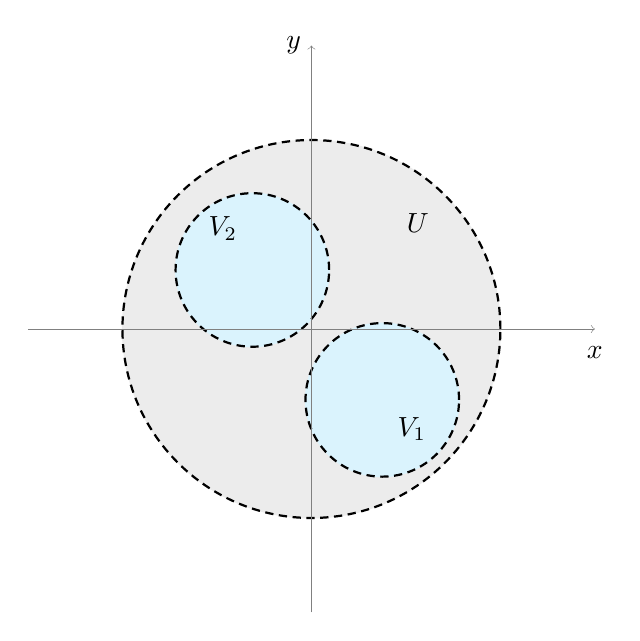
\begin{tikzpicture}[scale = 0.75]
            \def\gap{0.2}
            \def\bigradius{3.2}
            \def\smallradius{1.3}
            % \def\tinyradius
            
            \filldraw[gray!15] (0,0) circle (\bigradius cm);
            \draw[thick, densely dashed] (0,0) circle (\bigradius cm);
            
            \filldraw[ProcessBlue!15] (-1,1) circle (\smallradius cm);
            \draw[thick, densely dashed] (-1,1) circle (\smallradius cm);
        
            \filldraw[ProcessBlue!15] (1.2,-1.2) circle (\smallradius cm);
            \draw[thick, densely dashed] (1.2,-1.2) circle (\smallradius cm);
        
            % Axes
            \draw [help lines,->] (-1.5*\bigradius, 0) -- (1.5*\bigradius,0);
            \draw [help lines,->] (0, -1.5*\bigradius) -- (0,1.5*\bigradius);
            
            \node at (1.5*\bigradius,-0.4){$x$};
            \node at (-0.3, 1.5*\bigradius) {$y$};
        
            \node at (1.8, 1.8) {$U$};
            \node at (1.7, -1.7) {$V_1$};
            \node at (-1.5, 1.7) {$V_2$};
        
        \end{tikzpicture}
        \begin{tikzpicture}[scale = 0.75]
            \def\gap{0.2}
            \def\bigradius{3.2}
            \def\smallradius{1.3}
            % \def\tinyradius
            
            \filldraw[gray!15] (0,0) circle (\bigradius cm);
            \draw[thick, densely dashed] (0,0) circle (\bigradius cm);
            
            % \filldraw[ProcessBlue!15] (-1,1) circle (\smallradius cm);
            % \draw[thick, densely dashed] (-1,1) circle (\smallradius cm);
        
            % \filldraw[ProcessBlue!15] (1.2,-1.2) circle (\smallradius cm);
            % \draw[thick, densely dashed] (1.2,-1.2) circle (\smallradius cm);
        
            \begin{scope}[scale = 0.74]
                \filldraw[ProcessBlue!15] plot[smooth, tension=.7, closed hobby] coordinates {
                (-2.1,1.5) (-1,2.5) (1.5,1) (4,0.5) (3,-0.5) (2.5,-3)
                (0,-0.2) (-3,-2.5)};
                \draw[densely dashed, thick] plot[smooth, tension=.7, closed hobby] coordinates {
                (-2.1,1.5) (-1,2.5) (1.5,1) (4,0.5) (3,-0.5) (2.5,-3)
                (0,-0.2) (-3,-2.5)};
            \end{scope}
        
            % Axes
            \draw [help lines,->] (-1.5*\bigradius, 0) -- (1.5*\bigradius,0);
            \draw [help lines,->] (0, -1.5*\bigradius) -- (0,1.5*\bigradius);
            
            \node at (1.5*\bigradius,-0.4){$x$};
            \node at (-0.3, 1.5*\bigradius) {$y$};
        
            \node at (1.8, 1.8) {$U$};
            \node at (-2.1, -1.4) {$V$};
        \end{tikzpicture}        
    \end{center}
    On the left, we consider the set of all open sets contained in $V_1$ and $V_2$; this is a 
    sieve on the open disk (which we call $U$ to be consistent with our notation and discussion). 
    On the right, we consider the set of all open sets contained in the weirdly shaped $V$; this is 
    also a sieve on $U$. 
\end{example}

Some important facts about sieves on topological spaces that will be of interest to us.
\begin{itemize}
    \item Every open set $V \subset U$ corresponds to a sieve, which we call a \textbf{principal sieve}. 
    This sieve is simply the set of all open $V'$ contained in $V$. In the previous example, 
    the weirdly shaped region inside the open disk at the origin is a principal sieve.

    \item Every open cover of $\mathcal{U} = \{U_i\}_{i \in \lambda}$
    creates a \textbf{covering sieve} $S_{\mathcal{U}}$. This sieve is the set of all open $V$ such that $V \subset U_i$ 
    for some $i$, and where $V' \subset V$ implies $V'$ is also in the set. 
    
    Additionally, a covering sieve induces a (fairly stupid) functor
    $\mathcal{S}$, where:
    \[
        \mathcal{S}: \textbf{Open}(X)\op \to \textbf{Set}
        \qquad
        \mathcal{S}(V) 
        = 
        \begin{cases}
            \{\bullet\} & \text{If } V \in S_{\mathcal{U}}\\
            \varnothing & \text{ otherwise.}
        \end{cases}
    \]    
\end{itemize}

We are now prepared to continue our discussion. Our goal now will be to express 
the equalizer $E$ of $p, q$ categorically (i.e., without reference to its elements).
Let $P: \mathcal{O}(X)\op \to \textbf{Set}$ be a presheaf. Given an open set 
$U$ with open cover $\mathcal{U} = \{U_i\}_{i \in \lambda}$, we may construct 
$p, q$ using $\mathcal{U}$ as before, and take their equalizer $E$:
\begin{center}
    \begin{tikzcd}[column sep = 1.4cm, row sep = 1.4cm]
        E \arrow[r, "e"]
        &
        \displaystyle{\prod_{i \in \lambda}P(U_i)}
        \arrow[r, shift right = 0.5ex,swap, "p"]
        \arrow[r, shift right = -0.5ex, "q"]
        &
        \displaystyle{\prod_{i,j \in \lambda}P(U_i \cap U_j) }.
    \end{tikzcd}
\end{center}

We now prove the following result. 
\begin{lemma}
    Let $E$ be the equalizer of $p, q$ constructed using an open cover $\mathcal{U}$ of $U$. 
    Let $\mathcal{S}$ be the sieve functor induced by $\mathcal{U}$. Then
    \[
        E \cong \hom(\mathcal{S}, P) \quad \text{ or, in alternate notation, } \quad E \cong \text{Nat}(\mathcal{S}, P)
    \]
    That is, there is a bijection between $E$ and all natural transformations between $\mathcal{S}$ and $P$. 
\end{lemma}

\begin{prf}
    We know that 
    \[
        E = \Bigg\{(h_i)_{i \in \lambda} \Bigm\vert h_i|_{U_i \cap U_j} = h_j|_{U_i \cap U_j} \text{ for all } i, j \Bigg\}.
    \]
    We'll show that every $(h_i)_{i \in \lambda}$ can be used to build 
    a natural transformation between $\mathcal{S} \to P$. Showing the other direction 
    is not hard.

    Let $S_{\mathcal{U}}$ be our covering sieve induced by $\mathcal{U}$.
    Consider an element $(h_i)_{i \in \lambda}$ in $E$. For each $V \in S_{\mathcal{U}}$, 
    we define $h_V \in P(V)$ as
    \[
        h_V = h_i|_{V}
    \]
    where $i$ is the index such that $V \subset U_i$. Of course at least one index exists, 
    but it might not be the only index. Thus, a natural objection to this definition is the following 
    question: What if $V$ is contained in $U_i$ and $U_j$ for distinct $i$, $j$? 
    In this case, how do we define $h_V$?
    
    \begin{center}
        \begin{tikzpicture}[scale=1.5]
            \def\shapeone{%\draw[fill = red!40, draw = black, thick] 
            plot[smooth, tension=.5, closed hobby] coordinates {
                (4.6, 8.1) (3.5, 8.5) (2.2, 7.4) (2.4, 6.3) (3.8, 6.8) (4.9, 6.4) (5.3, 7.7) 
            };}
            \def\shapetwo{%\draw[fill = blue!40, draw = black, thick] 
            plot[smooth, tension = 0.5, closed hobby] coordinates {
                (3.5, 7.8) (4.1, 6.6) (5.6, 5.7) (6.7, 6.6) (6.4, 8.2) (5, 9) (4.2, 8.9)
            };}
            \def\shapethree{
            plot[smooth, tension = 0.3, closed hobby] coordinates {
            % (3.9, 8.3) (3.8, 7.7) (4, 7.1) (4.7, 6.9) (4.6, 7.6) 
            (3.9, 8.2) (3.8, 7.6) (4, 7) (4.7, 6.8) (4.6, 7.5)
            };
            }
            \fill[red!20] \shapeone;
            \fill[blue!20] \shapetwo;
    
            \begin{scope}
                \clip \shapeone;
                \fill[purple!30] \shapetwo;
            \end{scope}
    
            \fill[ProcessBlue!15] \shapethree;
            \draw \shapeone;
            \draw \shapetwo;
            \draw \shapethree;
    
            \node at (4.1, 8) {$V$};
            \node at (2.5, 6.5) {$U_i$};
            \node at (6.2, 6.5) {$U_j$};        
        \end{tikzpicture}
    \end{center}
    If $(h_i)_{i \in \lambda} \in E$, then we know that 
    agreement on the overlaps is guaranteed and so we may unambiguously 
    write $h_i|_V = h_j|_V = h_V$. 
    Hence, each $V \in S_{\mathcal{U}}$ corresponds to some \emph{unique} $h_V \in P(V)$
    for every $(h_i)_{i \in \lambda} \in E$. Furthermore, 
    we know that if $V' \subset V$, then $h_V|_{V'} = h_{V'}$.
    
    These facts allow us to create the following natural transformation 
    $\theta: \mathcal{S} \to P$ using an element $(h_i)_{i \in \lambda}$ of $E$, 
    as follows. 
    \begin{itemize}
        \item If $V \in S_{\mathcal{U}}$, we write $\theta_V: \{\bullet\} \to P(V)$ 
        where $\theta_V(\bullet) = h_V$, the unique $h_V$ we already know exists. 
    \end{itemize}
    This allows us to create the function 
    \[
        \phi: E \to \hom(\mathcal{S}, P) \qquad \phi\Big( (h_i)_{i \in \lambda} \Big) \mapsto (\theta: \mathcal{S} \to P)
    \]
    It is not difficult to show that every natural transformation between $\mathcal{S}$ and $P$ 
    corresponds to a unique element in $E$, thereby giving us an inverse to this function. Thus we have 
    our result.
\end{prf}

The above result is key to the the following proposition, which is what allows us 
to speak of a sheaf more abstractly. Before we introduce the proposition, we make a few 
comments.
\begin{itemize}
    \item Let 
\end{itemize}

\begin{proposition}
    Let $P: \textbf{Open}(X)\op \to \textbf{Set}$ be a presheaf. 
    Then $P$ is a presheaf if and only if
    for every open set $U$ and covering sieve $S$ of $U$, 
\end{proposition}



\newpage
\section{Stalks and Germs}
Let $(I, \le)$ be a partially ordered set, and suppose we have a functor 
$F: I \to \textbf{Set}$. With this functor, denote $F(i) = A_i$ and 
when $i \le j$, $F(i \le j) = f_{ij}: A_i\to A_j$. 
The limit of this functor $\displaystyle \Limto_{i \in I} F$ will be a set 
$A$ equipped with functions $\phi_i: A_i \to A$ with the universal property displayed below. 
\begin{center}
    \begin{tikzcd}[column sep = 1.4cm,  row sep = 1.4cm]
        A_{i} \arrow[rr, "f_{ij}"]
        \arrow[dr, swap, "\phi_i"]
        \arrow[ddr, swap, bend right, "\psi_i"]
        &
        &
        A_{j}
        \arrow[dl, "\phi_j"]
        \arrow[ddl, bend left, "\psi_j"]
        \\
        &
        A
        \arrow[d, dashed]
        &
        \\
        &
        K
        &
    \end{tikzcd}
\end{center}
We may naively suppose that $\displaystyle A = \coprod_{i \in I}A_i = \{(a, i) \mid a \in A_i, i \in I \}$, since such a set 
admits a family of functions $\displaystyle \text{inc}_i: A_i \to \coprod_{i \in I}A_i$. 
However, we cannot guarantee that this the triangle 
\begin{center}
    \begin{tikzcd}[column sep = 1cm,  row sep = 1.4cm]
        A_{i} \arrow[rr, "f_{ij}"]
        \arrow[dr, swap, "\text{inc}_i"]
        &
        &
        A_{j}
        \arrow[dl, "\text{inc}_j"]
        \\
        &
        {\displaystyle \coprod_{i\in I}A_i}
    \end{tikzcd}
\end{center}
will commute. In fact, it will never commute, since it would imply that 
for each $a \in A_i$, $(a, i) = (f_{ij}(a), j)$, which cannot happen as the 
tuples are mismatched. Since it is too strong to demand equality, we can define 
an equivalence relation $\sim$ on $\displaystyle \coprod_{i \in I}A_i$ 
as follows: For $i \le  j$, we say $(a, i) \sim (b, j)$ if 
$b = f_{ij}(a)$. We can then set 
\[
    A = \coprod_{i \in I}A_i \Big/\sim  
\]
and define a family of maps $\phi_i: A_i \to A$ which maps each $a \in A_i$ to 
its equivalence class under this relation. This then allows the desired triangle 
to commute and satisfies the universal property necessary for it to be the limit. 

We now apply this construction to our story with sheaves. 
\begin{definition}
    Let $X$ be a topological 
    space and $F: \mathcal{O}(X) \to \textbf{Set}$ a sheaf. For any point $x \in X$, 
    we define the \textbf{stalk of $F$ in $x$}, denoted $F_x$, 
    as the colimit 
    \[
        \Limto_{x \in U} F(U).
    \]
\end{definition}
The above notation is a bit informal, but many people use it, so we 
will stick with it and explicitly
describe this limit as follows. Each point $x \in X$ 
induces a functor $F^{(x)}: \mathcal{O}(X)_x \to \textbf{Set}$ where 
$\mathcal{O}_x$ is the category of open sets of $X$ \emph{containing} $x$, 
and $F^{(x)}(U) = F(U)$. We can then more formally say 
\[
    \Limto_{x \in U} F(U) =  \Limto_{U \in \mathcal{O}(X)_x}F^{(x)}.
\]
Therefore, we can say that 
\[
    \Limto_{x \in U} F(U) = \coprod_{U \mid x \in U}  F(U)\Big/\sim
\]
where $\sim$ is the equivalence relation described previously. In this instance, the equivalence relation translates 
as follows. Let $U_1 \subset U_2$ be two open sets. Then we say 
$(f, U_1) \sim (g, U_2)$ if $g\Big|_{U_1} = f$. 

We can make this more refined as follows. Let $U_1, U_2$ be more generally 
any two open sets such that $V = U_1 \cap U_2 \ne \varnothing$. 
Then clearly $V \subset U_1$ and $V \subset U_2$. 
Now suppose, $(f, V) \sim (g_1, U_1)$ for some $f, g_1$, and 
$(f, V) \sim (g_2, U_2)$. Then we now have that 
\[
    (g_1, U_1) \sim (g_2, U_2) \iff g_1\Big|_{V} = g_2\Big|_{V}. 
\]
Thus we have translated our original equivalence relation into a more 
useful one. To summarize, we have that our stalk is the set
\[
    \Limto_{x \in U} F(U) = \Bigg\{ \,[(f, U)] \mid x \in U \text{ open}, f \in F(U), \Bigg\}
\] 
where $(f, U)$ is a representative of its equivalence class $[(f, U)]$, 
described explicitly as
\[
    [(f, U)] = \Big\{ (g, V) \mid g \in F(U), x \in V \text{ open} \text{ and } g\Big|_{V} = f\Big|_{V}  \Big\}.
\]
The above line leads to our next definition. 

\begin{definition}
    Let $U$ be an open set containing $x$. There naturally exists projection map 
    \[
        \pi_U: F(U) \to F_x \qquad f \mapsto [(f, U)].
    \]
    Therefore, for each $f \in F(U)$, we define  
    the \textbf{germ of $f$ in $x$} to be the equivalence class 
    $[(f, U)]$ in the stalk $F_x$. 
\end{definition}

